\documentclass[10pt,a4paper,landscape]{article}
\usepackage{bib/trymtex}  % Using the custom trymtex package
\usepackage{multicol} % For multi-column layout
\usepackage{xcolor} % For additional colors
\usepackage{fancybox} % For boxed content
\usepackage{wasysym} % For additional symbols

% Set up for a tighter layout with less space wastage
\setlength{\parindent}{0pt}
\setlength{\parskip}{1pt}
\setlength{\columnsep}{10pt}
\setlength{\marginparwidth}{0pt}
\setlength{\marginparsep}{0pt}

% Page layout for the cheat sheet - maximize space
\geometry{top=0.4in, bottom=0.4in, left=0.4in, right=0.4in}


% Custom commands for better formatting
\newcommand{\sheader}[1]{%
  \vspace{1mm}
  \noindent{\large\color{sectioncolor}\textbf{#1}}
  \vspace{0.5mm}\\[-0.5em]
  \rule{\linewidth}{1pt}
  \vspace{0.5mm}
}

\newcommand{\ssubheader}[1]{%
  \vspace{0.5mm}
  \noindent{\normalsize\color{subsectioncolor}\textbf{#1}}
  \vspace{0.2mm}
}

\newcommand{\concept}[2]{%
  \vspace{0.5mm}
  \noindent\textbf{#1:} #2
  \vspace{0.2mm}
}

\newcommand{\alert}[1]{%
  \textcolor{alertcolor}{\textbf{#1}}
}

\newcommand{\tip}[1]{%
  \textcolor{tipcolor}{\textit{#1}}
}


% Title
\title{{\LARGE\color{titlecolor}\textbf{Numerical Solution of Differential Equations}}\\[0.1em]
      {\large\textit{TMA4212 Comprehensive Cheat Sheet}}}
\author{}
\date{}

\begin{document}
\thispagestyle{empty}
\maketitle
\vspace{-1.4cm}

\begin{multicols}{3}

%----------------------------------------------------------------------------------------
% FDM SECTION - THEORY
%----------------------------------------------------------------------------------------

\sheader{Finite Difference Methods (FDM)}

\ssubheader{Core Differentiation Operators}

\begin{formulabox}{Basic Operators}{basic-op}
$\Delta_h u(x) = u(x+h) - u(x)$ \hfill (Forward) \\
$\nabla_h u(x) = u(x) - u(x-h)$ \hfill (Backward) \\
$\delta_h u(x) = u(x+h) - u(x-h)$ \hfill (Central) \\
$\delta_h^2 u(x) = u(x+h) - 2u(x) + u(x-h)$ \hfill (2nd order)
\end{formulabox}

\begin{formulabox}{Approximations with Error Terms}{approx-op}
$\frac{\Delta_h u(x)}{h} = u'(x) + \frac{h}{2}u''(x) + O(h^2)$ \\
$\frac{\nabla_h u(x)}{h} = u'(x) - \frac{h}{2}u''(x) + O(h^2)$ \\
$\frac{\delta_h u(x)}{2h} = u'(x) + O(h^2)$ \\
$\frac{\delta_h^2 u(x)}{h^2} = u''(x) + O(h^2)$
\end{formulabox}

\begin{center}
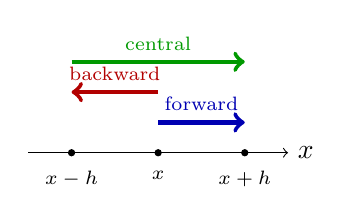
\begin{tikzpicture}[scale=0.55]
    % Number line
    \draw[->] (0,0) -- (6,0) node[right] {$x$};
    
    % Points and labels
    \foreach \x/\label in {1/x-h, 3/x, 5/x+h} {
        \filldraw[black] (\x,0) circle (2pt);
        \node[below] at (\x,-0.2) {\scriptsize $\label$};
    }
    
    % Forward difference
    \draw[blue!70!black, ->, ultra thick] (3,0.7) -- (5,0.7) node[midway, above] {\scriptsize forward};
    
    % Backward difference
    \draw[red!70!black, ->, ultra thick] (3,1.4) -- (1,1.4) node[midway, above] {\scriptsize backward};
    
    % Central difference
    \draw[green!60!black, ->, ultra thick] (1,2.1) -- (5,2.1) node[midway, above] {\scriptsize central};
\end{tikzpicture}
\end{center}

\ssubheader{Higher-Order Formulas}

\begin{formulabox}{$4^{th}$ Order Central Differences}{high-order}
$u'(x) \approx \frac{-u(x+2h) + 8u(x+h) - 8u(x-h) + u(x-2h)}{12h}$ \\[0.5em]
$u''(x) \approx \frac{-u(x+2h) + 16u(x+h) - 30u(x) + 16u(x-h) - u(x-2h)}{12h^2}$
\end{formulabox}

\begin{formulabox}{Compact FD Coefficients}{fd-coeffs}
\small
\begin{tabular}{|c|c|ccccc|}
\hline
Deriv. & Accuracy & \multicolumn{5}{c|}{Stencil Points} \\
 & & -2 & -1 & 0 & +1 & +2 \\
\hline
\multirow{3}{*}{$f'$} & $O(h)$ & - & - & -1 & 1 & - \\
& $O(h^2)$ & - & -1/2 & 0 & 1/2 & - \\
& $O(h^4)$ & 1/12 & -2/3 & 0 & 2/3 & -1/12 \\
\hline
\multirow{2}{*}{$f''$} & $O(h^2)$ & - & 1 & -2 & 1 & - \\
& $O(h^4)$ & -1/12 & 4/3 & -5/2 & 4/3 & -1/12 \\
\hline
\end{tabular}
\end{formulabox}

\ssubheader{Stability Analysis}

\begin{formulabox}{von Neumann Analysis}{von-neumann}
\textbf{Ansatz:} $u_j^n = \xi^n e^{ij\theta}$ where $\xi = \xi(\theta)$ \\
\textbf{Stability condition:} $|\xi(\theta)| \leq 1$ for all $\theta \in [-\pi, \pi]$ \\
\textbf{Plotting method:} Graph $|\xi(\theta)|$ vs $\theta$ for fixed $\frac{\Delta t}{\Delta x}$
\end{formulabox}

\begin{formulabox}{Matrix Stability}{matrix-stab}
For $\vec{u}^{n+1} = A\vec{u}^n$, stability requires: \\
$\rho(A) \leq 1$ (spectral radius condition) \\[0.5em]
\textbf{Types of stability:} \\
$\bullet$ $\rho(A) < 1$: asymptotically stable \\
$\bullet$ $\rho(A) = 1$ (simple): neutrally stable \\
$\bullet$ $\rho(A) > 1$: unstable
\end{formulabox}

\begin{formulabox}{CFL Condition Summary}{cfl}
\textbf{Advection equation} $u_t + au_x = 0$: \\
$C = \frac{|a|\Delta t}{\Delta x} \leq 1$ \\[0.5em]

\textbf{Diffusion equation} $u_t = \alpha u_{xx}$: \\
$r = \frac{\alpha \Delta t}{\Delta x^2} \leq \frac{1}{2}$ \\[0.5em]

\textbf{2D Advection:} \\
$\Delta t \left(\frac{|u_x|}{\Delta x} + \frac{|u_y|}{\Delta y}\right) \leq 1$ \\[0.5em]

\textbf{2D Diffusion:} \\
$\alpha\Delta t \left(\frac{1}{\Delta x^2} + \frac{1}{\Delta y^2}\right) \leq \frac{1}{2}$
\end{formulabox}

\begin{center}
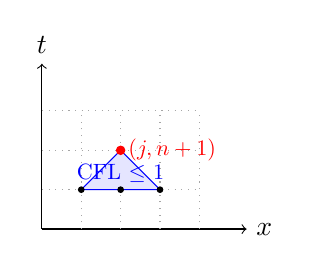
\begin{tikzpicture}[scale=0.5]
    % x/t grid
    \draw[->] (0,0) -- (5.2,0) node[right] {$x$};
    \draw[->] (0,0) -- (0,4.2) node[above] {$t$};
    
    % Grid lines
    \foreach \x in {1,2,...,4} {
        \draw[dotted, gray!70] (\x,0) -- (\x,3);
    }
    \foreach \y in {1,2,3} {
        \draw[dotted, gray!70] (0,\y) -- (4,\y);
    }
    
    % Domain of dependence
    \draw[blue, fill=blue!10] (2,2) -- (1,1) -- (3,1) -- cycle;
    \node[blue, scale=0.8] at (2,1.4) {CFL $\leq$ 1};
    
    % Current point
    \filldraw[red] (2,2) circle (3pt);
    \node[red, right, scale=0.8] at (2,2) {$(j,n+1)$};
    
    % Previous points
    \filldraw[black] (1,1) circle (2pt);
    \filldraw[black] (2,1) circle (2pt);
    \filldraw[black] (3,1) circle (2pt);
\end{tikzpicture}
\end{center}

%----------------------------------------------------------------------------------------
% FDM SECTION - APPLICATION
%----------------------------------------------------------------------------------------

\sheader{FDM Step-by-Step Process}

\begin{codebox}{Solving Elliptic PDEs (Poisson)}{elliptic-steps}
1. \textbf{Discretize domain}: $x_i = a + i\Delta x$, $y_j = b + j\Delta y$ \\
2. \textbf{Discretize operators}: e.g., $\nabla^2 u \approx \frac{u_{i+1,j} + u_{i-1,j} + u_{i,j+1} + u_{i,j-1} - 4u_{i,j}}{h^2}$ \\
3. \textbf{Apply boundary conditions}: Modify equations at boundary nodes \\
4. \textbf{Form linear system}: $AU = b$ \\
5. \textbf{Solve}: Direct or iterative method \\
6. \textbf{Analyze error}: Compute $\mathcal{O}(h^p)$ convergence rate
\end{codebox}

\begin{formulabox}{2D Poisson Equation}{poisson-2d}
\textbf{PDE:} $-\nabla^2 u = f$ in $\Omega$, $u = g$ on $\partial\Omega$ \\[0.5em]
\textbf{5-point stencil:} 
$-\frac{u_{i+1,j} + u_{i-1,j} + u_{i,j+1} + u_{i,j-1} - 4u_{i,j}}{h^2} = f_{i,j}$ \\[0.5em]
\textbf{Matrix form:} $AU = F$ with $A$ pentadiagonal
\end{formulabox}

\begin{center}
\small
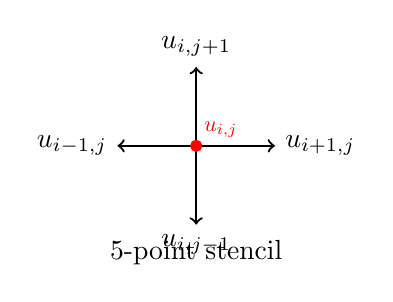
\begin{tikzpicture}[scale=0.5]
    % 5-point stencil
    \draw[->, thick] (0,0) -- (0,2) node[above] {$u_{i,j+1}$};
    \draw[->, thick] (0,0) -- (2,0) node[right] {$u_{i+1,j}$};
    \draw[->, thick] (0,0) -- (0,-2) node[below] {$u_{i,j-1}$};
    \draw[->, thick] (0,0) -- (-2,0) node[left] {$u_{i-1,j}$};
    \filldraw[red] (0,0) circle (4pt) node[above right, scale=0.8] {$u_{i,j}$};
    \node at (0,-2.7) {5-point stencil};
\end{tikzpicture}
\end{center}

\begin{codebox}{Solving Parabolic PDEs (Heat)}{parabolic-steps}
1. \textbf{Discretize}: $x_i = a + i\Delta x$, $t_n = n\Delta t$ \\
2. \textbf{Choose scheme}: 
   - Explicit (FTCS): $\frac{u_i^{n+1} - u_i^n}{\Delta t} = \alpha \frac{u_{i+1}^n - 2u_i^n + u_{i-1}^n}{\Delta x^2}$ \\
   - Implicit (BTCS): $\frac{u_i^{n+1} - u_i^n}{\Delta t} = \alpha \frac{u_{i+1}^{n+1} - 2u_i^{n+1} + u_{i-1}^{n+1}}{\Delta x^2}$ \\
   - Crank-Nicolson (CN): Average of FTCS and BTCS \\
3. \textbf{Apply conditions}: Initial and boundary \\
4. \textbf{Stability check}: $r = \frac{\alpha \Delta t}{\Delta x^2} \leq \frac{1}{2}$ (FTCS) \\
5. \textbf{Time-stepping}: March forward in time
\end{codebox}

\begin{formulabox}{Heat Equation Schemes}{heat-schemes}
\textbf{Heat equation:} $u_t = \alpha u_{xx}$ \\[0.5em]
\textbf{FTCS (Explicit):} 
$\frac{u_i^{n+1} - u_i^n}{\Delta t} = \alpha \frac{u_{i+1}^n - 2u_i^n + u_{i-1}^n}{\Delta x^2}$ \\[0.5em]
\textbf{BTCS (Implicit):} 
$\frac{u_i^{n+1} - u_i^n}{\Delta t} = \alpha \frac{u_{i+1}^{n+1} - 2u_i^{n+1} + u_{i-1}^{n+1}}{\Delta x^2}$ \\[0.5em]
\textbf{Crank-Nicolson:} 
$\frac{u_i^{n+1} - u_i^n}{\Delta t} = \frac{\alpha}{2} \left(\frac{u_{i+1}^{n+1} - 2u_i^{n+1} + u_{i-1}^{n+1}}{\Delta x^2} + \frac{u_{i+1}^n - 2u_i^n + u_{i-1}^n}{\Delta x^2}\right)$
\end{formulabox}

\begin{formulabox}{Stability for Heat Equation}{heat-stability}
\begin{tabular}{|c|c|c|c|}
\hline
\textbf{Scheme} & \textbf{Stability} & \textbf{Accuracy} & \textbf{Effort} \\
\hline
FTCS & $r \leq \frac{1}{2}$ & $O(\Delta t, \Delta x^2)$ & Low \\
BTCS & Unconditional & $O(\Delta t, \Delta x^2)$ & Medium \\
CN & Unconditional & $O(\Delta t^2, \Delta x^2)$ & High \\
\hline
\end{tabular}
\end{formulabox}

\begin{codebox}{Solving Hyperbolic PDEs (Wave)}{hyperbolic-steps}
1. \textbf{Discretize}: $x_i = a + i\Delta x$, $t_n = n\Delta t$ \\
2. \textbf{Choose scheme}: Consider characteristics \\
3. \textbf{Apply conditions}: Initial and boundary \\
4. \textbf{Stability check}: $C = \frac{c\Delta t}{\Delta x} \leq 1$ \\
5. \textbf{Time-stepping}: Use multi-level methods
\end{codebox}

\begin{formulabox}{Transport Equation Schemes}{transport}
\textbf{Transport equation:} $u_t + au_x = 0$ \\[0.5em]
\textbf{Upwind (for $a > 0$):} 
$\frac{u_i^{n+1} - u_i^n}{\Delta t} + a\frac{u_i^n - u_{i-1}^n}{\Delta x} = 0$ \\[0.5em]
\textbf{Lax-Friedrichs:} 
$\frac{u_i^{n+1} - \frac{1}{2}(u_{i+1}^n + u_{i-1}^n)}{\Delta t} + a\frac{u_{i+1}^n - u_{i-1}^n}{2\Delta x} = 0$ \\[0.5em]
\textbf{Lax-Wendroff:} 
$\frac{u_i^{n+1} - u_i^n}{\Delta t} + a\frac{u_{i+1}^n - u_{i-1}^n}{2\Delta x} = \frac{a^2\Delta t}{2}\frac{u_{i+1}^n - 2u_i^n + u_{i-1}^n}{\Delta x^2}$
\end{formulabox}

\begin{formulabox}{Stability for Transport Equation}{advection-stability}
\begin{tabular}{|c|c|c|c|}
\hline
\textbf{Scheme} & \textbf{Stability} & \textbf{Order} & \textbf{Properties} \\
\hline
Upwind & $C \leq 1$ & 1 & Diffusive \\
Lax-Friedrichs & $C \leq 1$ & 1 & Very diffusive \\
Lax-Wendroff & $C \leq 1$ & 2 & Dispersive \\
Leapfrog & $C \leq 1$ & 2 & Neutral, unstable \\
\hline
\end{tabular}
\end{formulabox}

%----------------------------------------------------------------------------------------
% FEM SECTION - THEORY
%----------------------------------------------------------------------------------------
\sheader{Finite Element Methods (FEM)}

\ssubheader{Key Concepts}

\begin{formulabox}{Weak Formulation}{weak-form}
\textbf{Strong form:} Find $u$ such that $Lu = f$ \\[0.5em]
\textbf{Weak form:} Find $u \in V$ such that \\
$a(u,v) = F(v) \quad \forall v \in V$ \\[0.5em]
where $a(u,v)$ is a bilinear form and $F(v)$ is a linear functional
\end{formulabox}

\begin{formulabox}{From Strong to Weak Form}{to-weak}
For $-\Delta u = f$ in $\Omega$ with $u=0$ on $\partial\Omega$: \\[0.5em]
1. Multiply by test function $v \in V$: $-\int_\Omega v\Delta u \, dx = \int_\Omega vf \, dx$ \\
2. Apply integration by parts: $\int_\Omega \nabla v \cdot \nabla u \, dx - \int_{\partial\Omega} v\frac{\partial u}{\partial n} \, ds = \int_\Omega vf \, dx$ \\
3. Use $v=0$ on $\partial\Omega$: $\int_\Omega \nabla v \cdot \nabla u \, dx = \int_\Omega vf \, dx$
\end{formulabox}

\begin{formulabox}{Galerkin Method}{galerkin}
\textbf{1. Choose finite-dimensional subspace} $V_h \subset V$ \\[0.5em]
\textbf{2. Approximate:} $u \approx u_h = \sum_{j=1}^n c_j \phi_j$ \\[0.5em]
\textbf{3. Form discrete problem:} Find $u_h \in V_h$ such that \\
$a(u_h,v_h) = F(v_h) \quad \forall v_h \in V_h$ \\[0.5em]
\textbf{4. Choose test functions:} $v_h = \phi_i$ for $i=1,\ldots,n$ \\[0.5em]
\textbf{5. Get linear system:} $\mathbf{K}\mathbf{c} = \mathbf{F}$ where \\
$K_{ij} = a(\phi_j,\phi_i)$ and $F_i = F(\phi_i)$
\end{formulabox}

\ssubheader{Function Spaces}

\begin{formulabox}{Sobolev Spaces}{sobolev}
$L^2(\Omega) = \{v : \int_\Omega v^2 \, dx < \infty\}$ \\[0.5em]
$H^1(\Omega) = \{v \in L^2(\Omega) : \nabla v \in [L^2(\Omega)]^d\}$ \\[0.5em]
$H^1_0(\Omega) = \{v \in H^1(\Omega) : v|_{\partial\Omega} = 0\}$ \\[0.5em]
$\|v\|_{H^1(\Omega)}^2 = \|v\|_{L^2(\Omega)}^2 + \|\nabla v\|_{L^2(\Omega)}^2$
\end{formulabox}

\ssubheader{Basis Functions}

\begin{formulabox}{1D Linear Elements}{linear-elements}
$\phi_i(x) = \begin{cases}
\frac{x-x_{i-1}}{h_i} & \text{for } x \in [x_{i-1}, x_i] \\
\frac{x_{i+1}-x}{h_{i+1}} & \text{for } x \in [x_i, x_{i+1}] \\
0 & \text{otherwise}
\end{cases}$ \\[0.5em]
with $\phi_i(x_j) = \delta_{ij}$ (Kronecker delta)
\end{formulabox}

\begin{formulabox}{2D Linear Elements}{2d-elements}
\textbf{On triangle with vertices $(x_1,y_1)$, $(x_2,y_2)$, $(x_3,y_3)$}: \\[0.5em]
$\phi_i(x,y) = a_i + b_i x + c_i y$ where $\phi_i(x_j,y_j) = \delta_{ij}$ \\[0.5em]
Or using barycentric coordinates $\lambda_1,\lambda_2,\lambda_3$: \\
$\phi_i(x,y) = \lambda_i(x,y)$
\end{formulabox}

\begin{center}
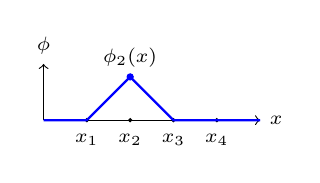
\begin{tikzpicture}[scale=0.55]
    % x-axis
    \draw[->] (0,0) -- (5,0) node[right] {\scriptsize $x$};
    \draw[->] (0,0) -- (0,1.3) node[above] {\scriptsize $\phi$};
    
    % Grid points
    \foreach \x in {1,2,3,4} {
        \filldraw[black] (\x,0) circle (1pt);
        \node[below] at (\x,-0.1) {\scriptsize $x_{\x}$};
    }
    
    % Hat function
    \draw[thick, blue] (0,0) -- (1,0) -- (2,1) -- (3,0) -- (5,0);
    \filldraw[blue] (2,1) circle (2pt);
    \node[above] at (2,1) {\scriptsize $\phi_2(x)$};
\end{tikzpicture}
\end{center}

\begin{formulabox}{Reference Elements}{reference-elements}
\textbf{Mapping from reference triangle $\hat{K}$ to physical element $K$:} \\
$F_K(\hat{x},\hat{y}) = 
\begin{pmatrix} x_1 \\ y_1 \end{pmatrix} +
\begin{pmatrix} 
x_2-x_1 & x_3-x_1 \\
y_2-y_1 & y_3-y_1
\end{pmatrix}
\begin{pmatrix} \hat{x} \\ \hat{y} \end{pmatrix}$ \\[0.5em]
\textbf{Jacobian of transformation:} \\
$J_K = \det\begin{pmatrix} 
x_2-x_1 & x_3-x_1 \\
y_2-y_1 & y_3-y_1
\end{pmatrix}$ \\[0.5em]
\textbf{Function transformation:} \\
$\phi(x,y) = \hat{\phi}(\hat{x},\hat{y})$
\end{formulabox}

%----------------------------------------------------------------------------------------
% FEM SECTION - APPLICATION
%----------------------------------------------------------------------------------------

\sheader{FEM Implementation Process}

\begin{codebox}{Step-by-Step FEM Process}{fem-steps}
1. \textbf{Define weak form}: Convert PDE to bilinear form \\
2. \textbf{Create mesh}: Triangulate domain $\Omega$ \\
3. \textbf{Choose finite element space}: $P_k$ elements \\
4. \textbf{Assemble linear system}: \\
   \quad $K_{ij} = a(\phi_j,\phi_i)$ and $F_i = F(\phi_i)$ \\
5. \textbf{Impose boundary conditions}: \\
   \quad Dirichlet: fix nodes directly \\
   \quad Neumann: include in weak form \\
6. \textbf{Solve system}: $\mathbf{Ku} = \mathbf{F}$ \\
7. \textbf{Post-process}: Compute error, visualize
\end{codebox}

\begin{formulabox}{Local Element Matrices}{local-matrices}
\textbf{For Poisson equation on a triangle $K$:} \\[0.5em]
\textbf{Element stiffness matrix:} \\
$A^K_{ij} = \int_K \nabla \phi_i \cdot \nabla \phi_j \, dK$ \\[0.5em]
\textbf{Element mass matrix:} \\
$M^K_{ij} = \int_K \phi_i \phi_j \, dK$ \\[0.5em]
\textbf{Element load vector:} \\
$F^K_i = \int_K f \phi_i \, dK$
\end{formulabox}

\begin{formulabox}{Quadrature Formulas}{quadrature}
\textbf{1D:} $\int_0^1 f(x) \, dx \approx \sum_{q=1}^Q w_q f(x_q)$ \\[0.5em]
\begin{tabular}{|c|c|c|c|}
\hline
\textbf{Rule} & \textbf{Points} & \textbf{Weights} & \textbf{Order} \\
\hline
Midpoint & $\{1/2\}$ & $\{1\}$ & 2 \\
Trapezoidal & $\{0,1\}$ & $\{1/2,1/2\}$ & 2 \\
Simpson & $\{0,1/2,1\}$ & $\{1/6,2/3,1/6\}$ & 4 \\
\hline
\end{tabular}\\[0.5em]
\textbf{Triangle:} $\int_K f(x,y) \, dK \approx |K| \sum_{q=1}^Q w_q f(x_q,y_q)$
\end{formulabox}

\begin{formulabox}{Assembly Process}{assembly}
\textbf{1. Compute local matrices} $A^K$ for each element \\[0.5em]
\textbf{2. Assembly by mapping local to global DOFs:} \\
For each element $K$ with local nodes $i,j$: \\
$A_{I(i),I(j)} \mathrel{+}= A^K_{ij}$ \\[0.5em]
where $I(i)$ is global index of local node $i$ \\[0.5em]
\textbf{3. Process boundary conditions:} \\
Dirichlet: $A_{i,:} = 0, A_{i,i} = 1, b_i = g_i$ \\
Neumann: Add boundary integral to $\mathbf{F}$
\end{formulabox}

%----------------------------------------------------------------------------------------
% IMPORTANT THEOREMS AND LEMMAS
%----------------------------------------------------------------------------------------

\sheader{Key Theorems \& Results}

\begin{formulabox}{Lax Equivalence Theorem}{lax-equiv}
For consistent numerical schemes: \\
\centerline{\alert{stability} $\Leftrightarrow$ \alert{convergence}}
\end{formulabox}

\begin{formulabox}{Lax-Milgram Theorem}{lax-milgram}
If $V$ is a Hilbert space and $a:V \times V \rightarrow \mathbb{R}$ is: \\
1. Continuous: $|a(u,v)| \leq M\|u\|_V\|v\|_V$ \\
2. Coercive: $a(v,v) \geq \alpha\|v\|^2_V$ with $\alpha > 0$ \\
Then for any bounded linear functional $F \in V'$: \\
$\exists$ unique $u \in V$ such that $a(u,v) = F(v)$ $\forall v \in V$ \\
Furthermore: $\|u\|_V \leq \frac{1}{\alpha}\|F\|_{V'}$
\end{formulabox}

\begin{formulabox}{Céa's Lemma}{cea}
Let $V_h \subset V$ be a finite-dimensional subspace. Then: \\
$\|u - u_h\|_V \leq C \inf_{v_h \in V_h} \|u - v_h\|_V$ \\
where $C$ is a constant independent of $h$.
\end{formulabox}

\end{multicols}
\end{document}